% !TEX root = ./Extended_Abstract.tex
%%%%%%%%%%%%%%%%%%%%%%%%%%%%%%%%%%%%%%%%%%%%%%%%%%%%%%%%%%%%%%%%%%%%%%%%
%                                                                      %
%     File: Extended_Abstract.tex                                      %
%     Tex Master: Thesis.tex                                           %
%                                                                      %
%     Author: Israel Sother                                            %
%     Last modified: 27 May 2024                                       %
%                                                                      %
%%%%%%%%%%%%%%%%%%%%%%%%%%%%%%%%%%%%%%%%%%%%%%%%%%%%%%%%%%%%%%%%%%%%%%%%
\documentclass[9pt,conference]{IEEEtran}
% \usepackage{cite}
\usepackage{amsmath,amssymb,amsfonts}
\usepackage{algorithmic}
\usepackage{graphicx}
\usepackage{textcomp}
\usepackage[table]{xcolor}
% Add prefix to references based on what is referred to
\usepackage[noabbrev]{cleveref}
\usepackage[numbers,sort&compress]{natbib} % <<<<< References in numbered list [1],[2],...
\usepackage{subfigure}
\usepackage{subcaption}
\usepackage{cancel}
\usepackage{subfigmat}
\usepackage{booktabs}
\usepackage{multirow}
\usepackage{microtype}

\begin{document}

\title{Real-time Ultra Short Horizon extension MPC for the control of a Formula Student Drive\\}

\author{\IEEEauthorblockN{Israel Sother}
\IEEEauthorblockA{israelsother@usp.br\\
\\ Instituto Superior Técninco, Lisboa, Portugal}
}

\maketitle
\thispagestyle{plain}
\pagestyle{plain}
\begin{abstract}
	This work presents the development of a control strategy for the motors of the Formula Student Team of Instituto Superior Técnico. The control strategy was developed with the main goal of improving the dynamic response of the motor torque and the system efficiency. The motor was experimentally characterized and a simulation environment was created to test different control strategies. The explicit Model Predictive Controller (MPC) was selected as the most suitable strategy due to its fast response and low current ripple. A novel horizon extension technique was proposed to reduce model mismatch, which gave the name of the controller: Real-time Ultra Short Horizon extension MPC (RUSH MPC). The control strategy was implemented in a Field Gate Programmable Array (FPGA) and a test bench setup was developed. The experimental results showed a close match with the simulation results, validating the torque estimation, the current measurements, and the control strategy. The system efficiency was improved due to the reduction in current Total Harmonic Distortion (THD) and the torque response was improved by orders of magnitude compared to the current solution.
\end{abstract}

\begin{IEEEkeywords}
Explicit MPC, Motor Control, Electric Vehicle, Formula Student, Horizon Extension.
\end{IEEEkeywords}

\section{Introduction}
With the increasing regulation efforts to reduce carbon footprints, an upward trend of investments in the mobility sector for the development of electric and hybrid powertrains has emerged. This field has received considerable interest for not only hardware improvements~\cite{Wang:power_converter_review:2020} but also new software alternatives with several new control strategies being proposed. From one side the advancing processing power available in microcontrollers has enabled the use of real-time predictive control strategies~\cite{Karamanakos:MPC_in_power_electronics:2020}, while the use of wide bandgap semiconductors results in a substantial efficiency improvement~\cite{Palmour:wide_bandgap_efficiency:2006}.

Formula Student is an engineering competition that challenges students to design, manufacture, and test a formula-style race car inside a given set of regulations. Similarly to the industry trend, the competition has pushed teams towards electrification, encouraging students to seek solutions that are lightweight, powerful, and efficient. The Formula Student Team of Técnico Lisboa (FST Lisboa) was funded in 2001, and since then has built 12 prototypes, from the fourth model (FST04) onward they have an electric powertrain, with the last 3 having autonomous racing mode.

A major advance in the power converter field was the use of wide bandgap semiconductors, which has allowed the development of more efficient converters with a higher power density. As a relatively new technology, there aren't many off-the-shelf solutions that fulfill the specifications required for a Formula Student prototype, thus some of the top teams started to develop their own motor drive solutions\@. FST started working on a fully self-developed powertrain in 2017 with motor development by~\citet{Sarrico:MSc}, and inverter development by Costa~\cite{Costa:MSc}. This development aligns with the fundamental objectives of Formula Student, which is empowering technical and practical knowledge to better prepare students. Additionally, the development of the entire powertrain system can result in a more efficient platform, creating a system optimized for each prototype. Unfortunately, the motor prototype is not ready to be used in the car, and the inverter is missing a system able to control the currently used motors. This work intends to fill a critical gap which is the absence of adequate control for a Permanent Magnet Synchronous Motor (PMSM). By developing and implementing a control strategy that enables the use of an in-house developed inverter with the commercial motor solution, this work not only addresses the identified bottleneck in the powertrain section but also shifts the performance envelope standards, improving the overall capabilities of the next prototypes.
\subsection{Topic Overview}
Through the years, several approaches have been proposed to control synchronous machines using a 2-level three-phase inverter. Regarding the control methods, several solutions have been presented in the literature with the most common being Field Oriented Control (FOC) and Direct Torque Control (DTC), with MDC~\cite{Bianchi:control_review} being introduced more recently, seeking a compromise between the advantages of FOC and DTC. Some approaches require a modulator such as Space Vector Modulation (SVM)~\cite{Neacsu:SVM_intro:2001:IECON}, while others can directly output the semiconductor trigger signals~\cite{Vazquez:MPC_in_power_systems_review:2017:IEEE}.

The use of FOC and DTC have dominated the market for many years due to their simple implementation, but each of them has downsides\@. FOC combined with current control PID is known for having a slow dynamic response when compared to DTC, while in steady-state behavior and disturbance rejection, FOC shows better results with smaller torque ripple and current THD~\cite{Merzoug:FOCvsDTC:2008,Korkmaz:FOCvsDTC:2013,Souad:FOCvsDTC:2008}. MPC has been proposed as a combination of the two, exhibiting a good dynamic response while being able to maintain low current and torque ripple. 

Technical advances in the microprocessor industry have allowed the increasing use of MPC in power converters and drives~\cite{Vazquez:MPC_in_power_systems_review:2017:IEEE}. This non-linear control scheme provides easy constraint integration while optimizing the control action in real time and is adaptable to different types of electric machines being controlled. The main downside of this strategy is the increased computational cost, which is offset by the decreased cost of computational power.

MPC in power systems is usually divided into two categories: Continuous Set MPC (CSMPC) and Finite Set MPC (FSMPC)~\cite{Wang:MPC_in_Electrical_Machines_review:2017:IEEE}, depending on their output signals. The first type calculates the best possible voltage vector and then uses a modulator like SVM to compose it, while FSMPC exploits the fact that a motor drive usually has a limited number of possible voltage vectors and thus predicts the currents for each of those vectors to evaluate the best option. The second approach usually doesn't need a modulator as it only considers the finite set of all possible converter states, although some variations have tried to increase the search space by introducing synthetic vectors that are created from a combination of the native ones. This technique of subdivision and refining vectors can be used to create a quasi-continuous set MPC~\cite{Ma:MPC_Syntetic_vector:2014:IEEE}, which, when combined with reducing the search area to the most probable sector, can improve the torque and current ripple without a prohibitive increase in computational cost.

\section{Teoretical Backgroung and PMSM Model}
This section briefly introduces the Formula Student competition structure and the general powertrain model used in this work.
\subsection{Formula Student}
In a formula student competition, two types of evaluation exist, the first category is comprised of static events where the design, cost, and business model of the prototype are analyzed. In the dynamic category, each prototype is evaluated through 5 different events: Skidpad, Acceleration, AutoX, Endurance, and Efficiency (evaluated in the Endurance track).  The skidpad event consists of two circles of radius 9.125m, where the vehicle follows an eight pattern. The acceleration event consists of a standing start 75m straight acceleration, with the maximum battery power limited to 80kw, as it is for all Formula Student events. The AutoX is a 1km track with several corners and straights mixed. The endurance event is similar to the AutoX, with enough laps to complete 22km. Lastly, the efficiency event is evaluated in the Endurance track, where the teams are scored based on the energy consumed to complete the 22km track and the time it took to complete it.

\subsection{Two Level Voltage Source Inverter}

The usual hardware used to control synchronous machines is a 2-level Voltage Source Inverter. Such equipment is composed of six switches organized in three legs, where each pair of switches is connected to a motor terminal, as shown in \Cref{fig:inverter_and_motor_schematic}.

\begin{figure}[!htb]
	\centering
	\includegraphics[width=0.9\linewidth]{Figures/Inverter.pdf}
	\caption[2-Level Voltage source Inverter arrangement.]{2-Level Voltage source Inverter arrangement.}
	\label{fig:inverter_and_motor_schematic}%chktex 24
\end{figure}

Usually, each switch in an inverter leg is operated with the inverse logic of the other switch in the leg, and this arrangement allows for 8 different switching combinations where 2 of them result in null voltages. That gives 7 possible voltage vectors, as detailed in \Cref{table:space_vector} and \Cref{fig:space_vector}. In \Cref{table:space_vector} the Vector column denotes the top switches states ($S_1$,$S_2$, and $S_3$), where a 1 means the top switch is the conducting state with the bottom switch is on a cut-off state and a 0 the opposite. The $\alpha$ and $\beta$ components which define the state space vectors are as defined by the Concordia transformation.
\begin{table}[h]
	\centering
	\caption{Space vector for a 2-level three-phase inverter}
	\label{table:space_vector}%chktex 24
	\renewcommand{\arraystretch}{1.7} % more space between rows
	% \resizebox{0.5\textwidth}{!}{%
		\begin{tabular}{|
				>{\columncolor[HTML]{E0E0E0}}c |
				>{\columncolor[HTML]{E0E0E0}}c |c|c|}
			\hline %chktex 44
			\cellcolor[HTML]{A0A0A0}\textbf{Switch State} &
			\cellcolor[HTML]{A0A0A0}\textbf{Vector}       &
			\cellcolor[HTML]{A0A0A0}\textbf{$V_{\alpha}$} &
			\cellcolor[HTML]{A0A0A0}\textbf{$V_{\beta}$}  \\ \hline %chktex 44
			0 & 000 & $0$                         & $0$                       \\ \hline %chktex 44
			1 & 001 & $\sqrt{\frac{2}{3}}V_{DC}$  & $0$                       \\ \hline %chktex 44
			2 & 010 & $\frac{1}{\sqrt{6}}V_{DC}$  & $\frac{1}{\sqrt{2}}V_{DC}$\\ \hline %chktex 44
			3 & 011 & $-\frac{1}{\sqrt{6}}V_{DC}$ & $\frac{1}{\sqrt{2}}V_{DC}$\\ \hline %chktex 44
			4 & 100 & $-\sqrt{\frac{2}{3}}V_{DC}$ & $0$                       \\ \hline %chktex 44
			5 & 101 & $-\frac{1}{\sqrt{6}}V_{DC}$ & $\frac{1}{\sqrt{2}}V_{DC}$\\ \hline %chktex 44
			6 & 110 & $\frac{1}{\sqrt{6}}V_{DC}$  & $\frac{1}{\sqrt{2}}V_{DC}$\\ \hline %chktex 44
			7 & 111 & $0$                         & $0$                       \\ \hline %chktex 44
		\end{tabular}%
	% }
\end{table}
\subsection{Space Vector Modulation}
\label{subsection:Space Vector Modulation}%chktex 24

Several modulation techniques have been proposed in the literature like Sinusoidal Pulse Width Modulation (SPWM), Selective Harmonic Elimination (SHE)~\cite{Asadzadeh:selective_harmonic_elimination:2019}, SVM~\cite{Neacsu:SVM_intro:2001:IECON}.
% , or \gls{svc}~\cite{An:space_vector_control:2016}. Some of these techniques are exclusive of multilevel inverters, like \gls{svc}~\cite{Rodriguez:svc_multilevel:2002}, while others also work for two-level inverters. 
The most common method of modulation in digital motor control is SVM, as it is a robust, easy-to-implement technique, and allows higher voltage ratio. 

% The figure "fig:space_vector" provides a visual representation of the space vector for a 2-level three-phase inverter. It shows the possible voltage states that can be applied to the motor. The phase voltages are represented in a 2D plane, with the maximum phase voltage shown by a circle. Any point within this circle is attainable without overmodulation or neutral point shift. The hexagon represents the maximum voltage that can be applied to the motor, and the vectors within the hexagon are the possible voltage states.
\Cref{fig:space_vector} shows a 2D representation of the space vector for a 2-level three-phase inverter. The basic voltage vectors (previously defined on \Cref{table:space_vector}) are shown pointing to the hexagon corners. 
% Note that they can only reach those voltages if modulation techniques that produce shifting in the neutral point (like third harmonic injection) are used.
 Connecting the basic vectors produces the hexagon of possible voltage states.

\begin{figure}[!htb]
	\centering
	\includegraphics[width=1\linewidth]{Figures/Space_Vector_revised.pdf}
	\caption[Space vector for a 2-level three-phase inverter.]{Space vector for a 2-level three-phase inverter.}
	\label{fig:space_vector}%chktex 24
\end{figure}


Using SVM it is possible to modulate any vector inside the hexagon shown in \Cref{fig:space_vector}, but if a pure sinusoidal output is desired, the vectors should be constrained to the inscribed circle, that has a radius of $\frac{1}{\sqrt{2}} V_{DC}$. The reason behind this is to keep the reference vector locus inside the hexagon, avoiding distortions in the output. Note that although it is possible to generate waveforms with higher RMS value, it is not possible to modulate a peak higher than $\frac{1}{\sqrt{2}} V_{DC}$ for every vector angle. If a higher RMS value is requested the generated voltage will be saturated on the sides of the hexagon while near the corners it will achieve the requested value, thus those waveforms become more and more distorted as the amplitude approaches $\sqrt{\frac{2}{3}} V_{DC}$. To modulate a sinusoidal output the vector should develop a circular trajectory, but in the overmodulation region the voltage constrains it to the voltage hexagon, and thus the difference between the intended and the effectively applied vector increases.

To modulate a voltage vector that is not exactly one of the basic voltage vectors a modulation technique is needed. When using the SVM method to compose a given reference vector $V_{ref}$, the algorithm first detects the sector on which the reference vector lays. With the sector identified a ratio between the adjacent basic vectors and a null vector is selected so that the average vector is equal to the reference vector. This ratio is calculated as shown in \Cref{eq:svm_vref}.

For example, let's consider the reference vector shown in \Cref{fig:space_vector}. According to SVM, this vector can be modulated by using $V_1$ for half of the active time and $V_3$ for the other half of the active time. The active time refers to the duration when the vector amplitude is non-zero, while the null time refers to the duration when a null vector is used to reduce the output amplitude. This modulation can be expressed by \Cref{eq:svm_vref}, where $T_1+T_3$ represents the active time and $T_{null}$ represents the null time.

\begin{equation}
	V_{ref} = \frac{T_{null} V_{null} + T_1 V_1  + T_3 V_3}{h}
	\label{eq:svm_vref}
\end{equation}

%% epxplanation of the neutral point shift. it should follow the following equation: V_shift = K_{shift}*max(V_{AN},V_{BN},V_{CN) + (1-K_{shift})*min(V_{AN},V_{BN},V_{CN)


% In the hardware implementation, the voltage reference is generated in the rotor reference frame (dq0) and then the inverse dq0 transformation is applied to obtain the phase voltages directly, without selecting a sector to know which vectors to use. These phase voltages are then divided by the DC link voltage to obtain the duty cycle of the switches. Note that this does not account though for the neutral point shift. This simplification results in the same switching times for the active vectors as the geometric approach of calculating which sector the reference vector is and then decomposing the reference vector in the two adjacent vectors. The null vector distribution between $V_0$ and $V_7$ will dictate the neutral point shifting method. 

% Several approaches have been proposed to accomplish this shift and they all rely on injecting a variable offset voltage on the neutral point that has a strong third harmonic component. Although a pure third harmonic sine wave can be used it is computationally expensive when compared with other methods such as top, mid, or bottom clamp. This technique of mid-clamp aims to center the neutral point between the DC link terminals, while the top clamp shifts the neutral point to the maximum voltage and the bottom clamp to the minimum voltage. The main advantage of a top or bottom clamp is the reduced number of switching events when compared with a mid-clamp. 

% The chosen approach is defined by \Cref{eq:neutral_point_shift}, where $K_{shift}$ is the shift factor, and $V_{AN}$,$V_{BN}$, and $V_{CN}$ are the phase voltages referenced to a virtual neutral point that is the average of the phase voltages with respect to the DC link negative terminal. The value of $K_{shift}$ dictates the shift method used, when it is equal to 1 the top-clamp method is used, if it is 0.5 then the mid-clamp is used, and 0 results in the bottom-clamp method.\~\citet{Microchip:ZSM_viewer:2023} has a visualization tool with the main methods shown. The calculated shift voltage is then summed to the desired phase voltages, and the modulation technique is applied as usual. In the implementation, this results in the MOSFETs dutty cycle being shifted to center at the value of $K_{shift}$.

% \begin{equation}
%     \begin{split}
% 	V_{shift} = K_{shift} - K_{shift} \max \left(V_{AN},V_{BN},V_{CN}\right) - \\ - (1-K_{shift}) \min \left(V_{AN},V_{BN},V_{CN}\right)
%     \end{split}
% 	\label{eq:neutral_point_shift}
% \end{equation}



\subsection{PMSM model}\label{section:PMSM model}
A model to represent the PMSM with delta-arranged windings is needed to develop the controller. The used model is a 3-phase model in a rotor reference frame (dq0), with permanent magnets on the rotor in a spoke arrangement. The model equations are shown in \Cref{eq:motor_with_inductances_no_derivative}, where $u_d$ and $u_q$ are the d and q components of the stator voltage, $r$ is the stator phase resistance, $L_d$ and $L_q$ are the d and q components of the stator inductance, $i_d$ and $i_q$ are the d and q components of the stator phase current, $\omega_e$ is the electrical angular velocity, $\psi_{PM}$ is the permanent magnet flux, $T_e$ is the electromagnetic torque, $T_{load}$ is the load torque, $T_{loss}$ is the total losses torque, and $J$ is the moment of inertia of the rotor. Note that the inductances are assumed to be a function of the current in the respective DQ0 component, this allows the model to account for saturation effects. This could be used to model also the cross-magnetization effect, but limitations in the implementation of the control strategy prevented this from being used. 

\begin{subequations}
	\begin{equation}
		% \left\{
		% \begin{aligned}
		u_d = r i_d+L_d\frac{d i_d}{dt} - \omega_e L_q i_q              \\
	\end{equation}
	\begin{equation}
		u_q = r i_q+L_q\frac{d i_q}{dt} + \omega_e (L_d i_d +\psi_{PM})
	\end{equation}
	\begin{equation}
		T_e  = p\, i_q(( L_d - L_q)i_d + \psi_{PM})                       \\ %= p( (L_d i_d + \psi_{PM}) i_q - L_q i_q i_d)
	\end{equation}
	\begin{equation}
		\frac{d\omega_e}{dt} = \frac{T_e-T_{load} - T_{loss}}{J}
	\end{equation}
	\begin{equation}
		\frac{d\theta_e}{dt} = \omega_e
		% \end{aligned}
		% \right.
	\end{equation}
	\label{eq:motor_with_inductances_no_derivative}
\end{subequations}

An approximation of the differential equations is needed to discretize the equations to be able to use the model in a discrete time control system. Two usual solutions are the Backward and the Forward Euler methods. Although simpler to compute, the Forward Euler method is prone to instabilities especially in fast systems such as power converters, in contrast with the Backward alternative that is unconditionally stable. Due to this consideration, the Euler Backward technique will be prioritized. Applying this method to \Cref{eq:motor_with_inductances_no_derivative} would result in an equation that has algebraic loops so to avoid that a few approximations were made. First, the inductance change due to current variation in a timestep $h$ is assumed to be small enough so that the inductances can be calculated using the previous time step currents ($ L_{x(i_x(k+1))} \approx L_{x(i_x(k+1))} $). Similarly, the rotor speed is assumed to vary little between iterations, so that $\omega_{(k+1)} \approx \omega_{(k)}$.

With those considerations, and rearranging the equations, the system can be solved iteratively, as shown in \Cref{eq:motor_backward_euler_matrix}.

\begin{subequations}
	\begin{equation}
		\begin{aligned}
			\begin{bmatrix}
				i_{d(k+1)} \\
				i_{q(k+1)} \\
			\end{bmatrix}
			=
			\begin{bmatrix}
				1                                                    & -h\frac{\omega_{e(k)}L_{q(i_q(k))}}{hr+L_{d(i_d(k))}} \\
				h\frac{\omega_{e(k)}L_{d(i_d(k))}}{hr+L_{q(i_q(k))}} & 1                                                     \\
			\end{bmatrix}^{-1} \\
			\left(
			\begin{bmatrix}
					\frac{L_{d(i_d(k))}}{hr+L_{d(i_d(k))}} & 0                                      \\
					0                                      & \frac{L_{q(i_q(k))}}{hr+L_{q(i_q(k))}} \\
				\end{bmatrix}
			\begin{bmatrix}
					i_{d(k)} \\
					i_{q(k)} \\
				\end{bmatrix}+\right. \\ +
			\begin{bmatrix}
					\frac{h}{hr+L_{d(i_d(k))}} & 0                          \\
					0                          & \frac{h}{hr+L_{q(i_q(k))}} \\
				\end{bmatrix}
			\begin{bmatrix}
					u_{d(k+1)} \\
					u_{q(k+1)} \\
				\end{bmatrix}
			+\\+\left.
			\begin{bmatrix}
					0                                                 \\
					-h\frac{\omega_{e(k)}\psi_{PM}}{hr+L_{q(i_q(k))}} \\
				\end{bmatrix}
			\right)
		\end{aligned}
	\end{equation}

	\begin{equation}
		T_{e(k+1)}  = p\, i_{q(k+1)}((L_{d(i_d(k+1))} - L_{q(i_q(k+1))})i_{d(k+1)} + \psi_{PM})
	\end{equation}

	\begin{equation}
		\begin{aligned}
			\begin{bmatrix}
				\omega_{e(k+1)} \\
				\theta_{e(k+1)}
			\end{bmatrix}
			=
			\begin{bmatrix}
				1 & 0 \\
				h & 1
			\end{bmatrix}
			\begin{bmatrix}
				\omega_{e(k)} \\
				\theta_{e(k)}
			\end{bmatrix}+\\+
			\frac{T_{e(k+1)}-T_{load(k+1)} - T_{loss(k+1)}}{J}
			\begin{bmatrix}
				h \\
				h^2
			\end{bmatrix}
		\end{aligned}
	\end{equation}
	\label{eq:motor_backward_euler_matrix}
\end{subequations}

\section{Motor characterization}
\label{section:motor_characterization}
Although AMK has provided the motor datasheet with the key parameters on it, it is important to verify how well they track the real values, and how they change regarding the motor operation. The datasheet values are linear approximations of the magnetic circuit on the motor, and as such do not accurately represent the machine at high current operating points. To account for the saturation effect, a variable inductance approach will be used~\cite{Wijenayake:saturation_model:1997,Stumberger:saturation_model:2003}, where the inductance of each axis will be a function of the current on the respective axis. 
\subsection{Phase Resistance}
Assuming the machine is well balanced, the phase resistance will be equal to $\frac{3}{2}$ of the terminal resistance. The phase resistance was measured using a micro-ohmmeter (\textit{UNI-T UT620A Micro-ohmmeter}), that has a resolution of $10\mu \Omega$ with an accuracy of $\pm (0.25\% + 25\mu \Omega)$. The measurements were taken on the terminal wires at room temperature and with the kelvin probe, resulting in $142.89 \pm 0.06 m\Omega$. This value is close to the datasheet one of $135 m\Omega$, and the difference is probably due to the wire terminals. The resultant phase resistance ($r$) is $214.335 \pm 0.091 m\Omega$.
\subsection{Flux Linkage}
The flux linkage was measured by connecting the rotor to an external motor that kept it at a constant known speed without any connection between the terminals, this ensures the current is zero as in \Cref{eq:flux_measuring}. Then an oscilloscope (\textit{Promax OD-571}) was connected to two terminal wires and used to measure the back EMF. The oscilloscope on the used settings has an accuracy of $\pm(3\% + 0.2508 V)$. This was repeated for several speeds, resulting in \Cref{fig:flux_linkage_rpm}.

\begin{subequations}
	\begin{equation}
		u_d = r_d \cancelto{0}{i_d}+\cancelto{0}{\frac{d i_d}{dt}}\left(L_d + \cancelto{0}{i_d}\frac{d L_d}{di_d}\right) - \omega_e L_q \cancelto{0}{i_q} = 0                \\
	\end{equation}
	\begin{equation}
		u_q = r_q \cancelto{0}{i_q}+ \cancelto{0}{\frac{d i_q}{dt}} \left(L_q + \cancelto{0}{i_q}\frac{d L_q}{di_q}\right) + \omega_e (L_d \cancelto{0}{i_d} +\psi_{PM})  = \omega_e \psi_{PM}\\
	\end{equation}
	\label{eq:flux_measuring}
\end{subequations}

\begin{figure}[!htb]
	\centering
	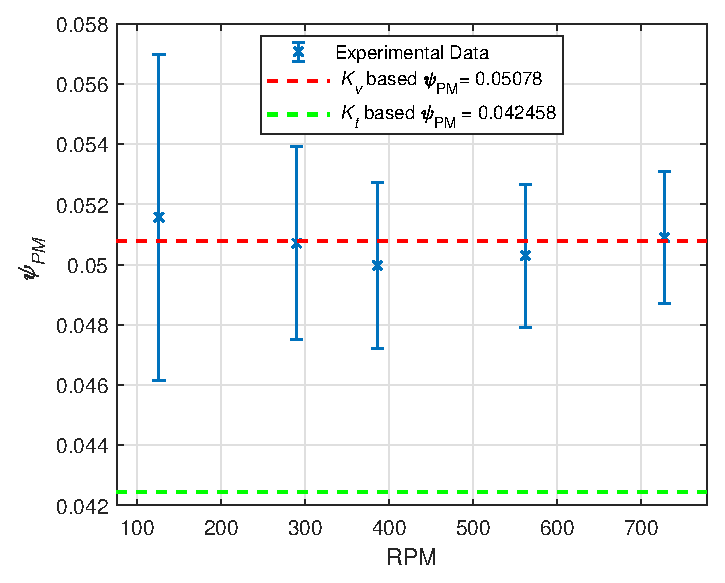
\includegraphics[width=0.4\textwidth]{Figures/Flux_test.eps}
	\caption[Flux Linkage as a function of RPM.]{Flux Linkage as a function of RPM.}
	\label{fig:flux_linkage_rpm} %chktex 24
\end{figure}

In this graph, two other lines are shown, they represent the flux linkage estimated using the torque and speed constant provided in the datasheet. Notice that the experimental data aligns well with the value derived from the voltage constant but it is very different from the value derived from the torque constant. This is probably due to different references and transformations being used, but as there isn't much information available on the datasheet, the measured value is assumed to be the correct one.
\subsection{ Machine direct and quadrature inductances}
The inductances were characterized according to~\citet{Stumberger:saturation_model:2003}. This method uses a Voltage Source Inverter coupled with a control algorithm to keep the current in one of the axes constant, and then do a voltage step in the other axis. The current is then integrated to obtain the current-induced flux linkage as shown in \Cref{eq:inductance_voltage_step}, and then the inductance is calculated as the derivative of the current-induced flux linkage.

The flux-induced curve is then approximated as a fit of several exponential curves, as this allows the inductance to be calculated as the analytical current derivative of this exponential fit. The current induced flux linkage and its exponential fit are shown in \Cref{fig:inductances_method_2}, and the inductance presented in \Cref{fig:inductance_time_constant}. 

\begin{subequations}
	\begin{equation}
		u_d = ri_d(t) + \frac{d\psi_d (t)}{dt} - \psi_q \cancelto{0}{\omega_e}
	\end{equation}
	\begin{equation}
		u_q = ri_q(t) + \frac{d\psi_q (t)}{dt} + \left(\psi_d + \psi_{PM}\right) \cancelto{0}{\omega_e}
	\end{equation}
\end{subequations}


\begin{subequations}
	\begin{equation}
		\frac{d\psi_d (t)}{dt} = u_d - ri_d(t)
	\end{equation}
	\begin{equation}
		\frac{d\psi_q (t)}{dt} = u_q - ri_q(t)
	\end{equation}
	\label{eq:inductance_voltage_step}
\end{subequations}

% \begin{figure}[!htb]
% 	\centering
% 	\includegraphics[width=0.6\textwidth]{Figures/id-5__vq-30.eps}
% 	\caption[Quadrature Flux linkage @$i_d = -5$A.]{Quadrature Flux linkage @$i_d = -5$A.}
% 	\label{fig:flux_linkage_curve} %chktex 24
% \end{figure}

% trim={<left> <lower> <right> <upper>}
\begin{figure}[!htb]
	\begin{subfigmatrix}{2}
		\subfigure[Flux Linkage d axis exponential fit.]{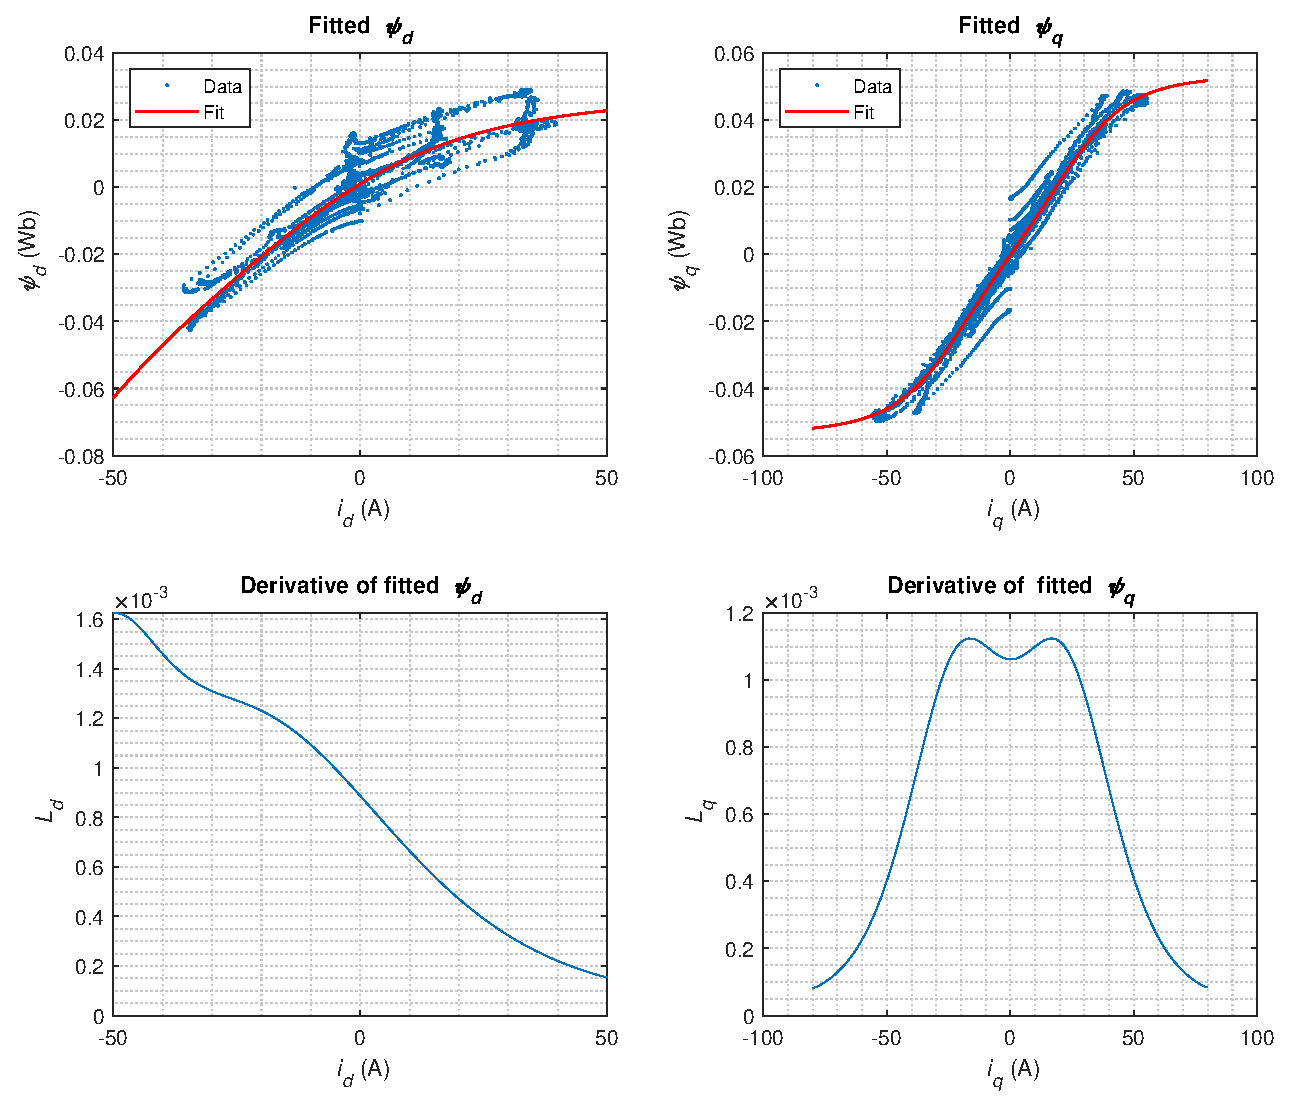
\includegraphics[clip, trim=0cm 9.5cm 11.1cm 0cm,width=0.45\linewidth]{Figures/Ldq.eps}}
		\subfigure[Flux Linkage q axis exponential fit.]{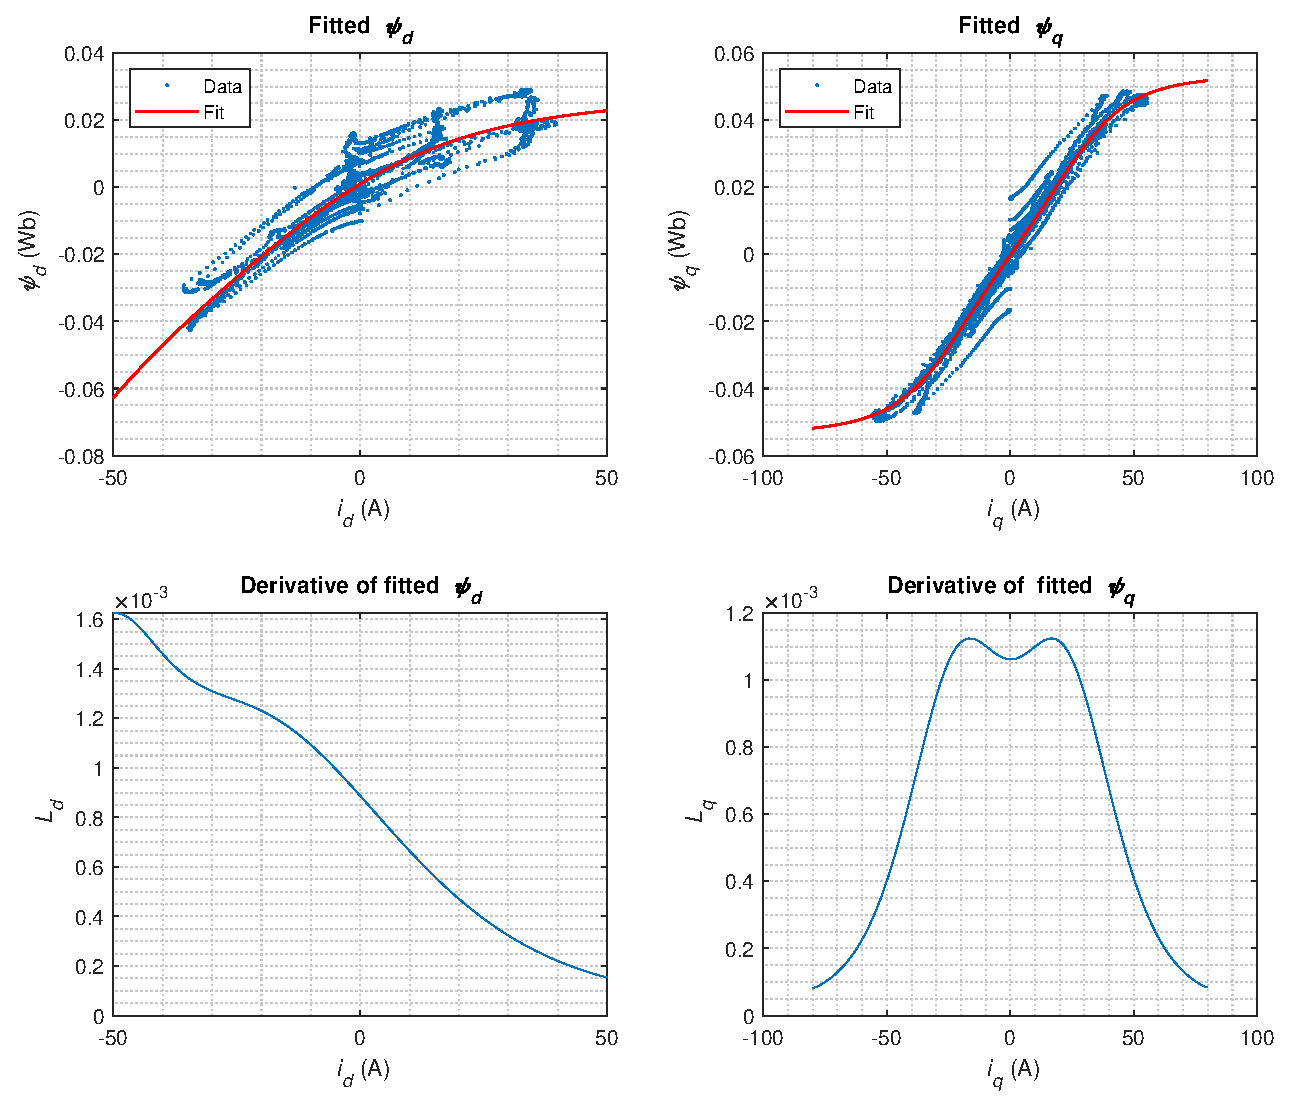
\includegraphics[clip, trim=11.1cm 9.5cm 0cm 0cm,width=0.45\linewidth]{Figures/Ldq.eps}}
	\end{subfigmatrix}
	\caption{Flux Linkage exponential fit. The blue dots are the measured flux linkage, while the red line is the exponential fit (R-square 0.8879 for $\psi_d$ and 0.9681 for $\psi_q$).}
	\label{fig:flux_linkage_fit}%chktex 24
\end{figure}

\begin{figure}[!htb]
	\begin{subfigmatrix}{2}
		\subfigure[Machine Inductance in d axis.]{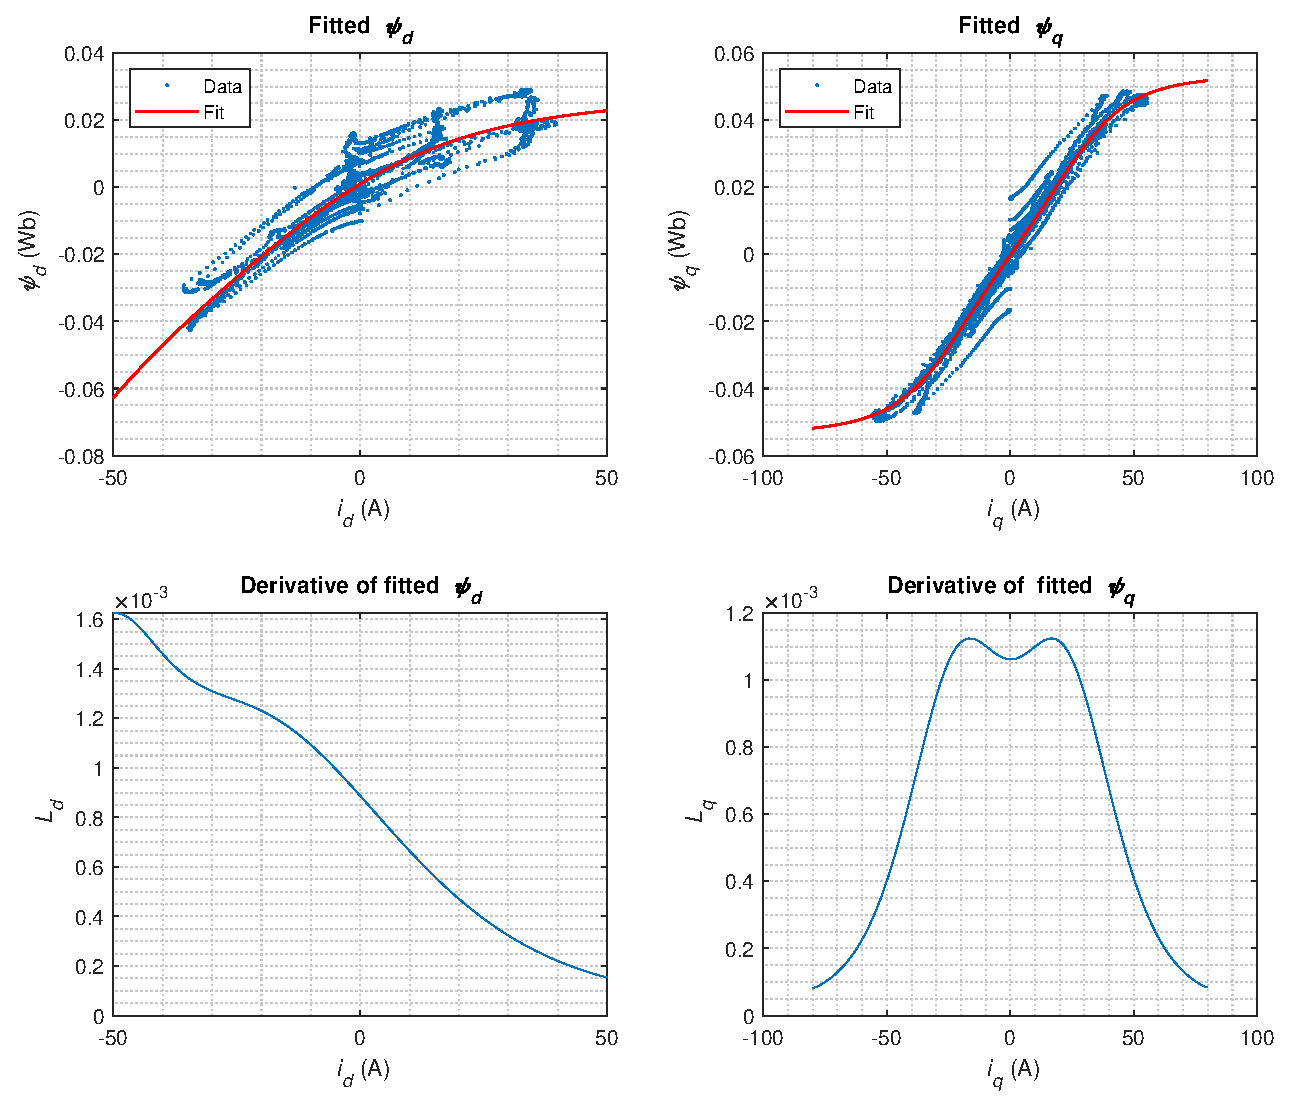
\includegraphics[clip, trim=0cm 0cm 11.1cm 10.1cm,width=0.45\linewidth]{Figures/Ldq.eps}}
		\subfigure[Machine Inductance in q axis.]{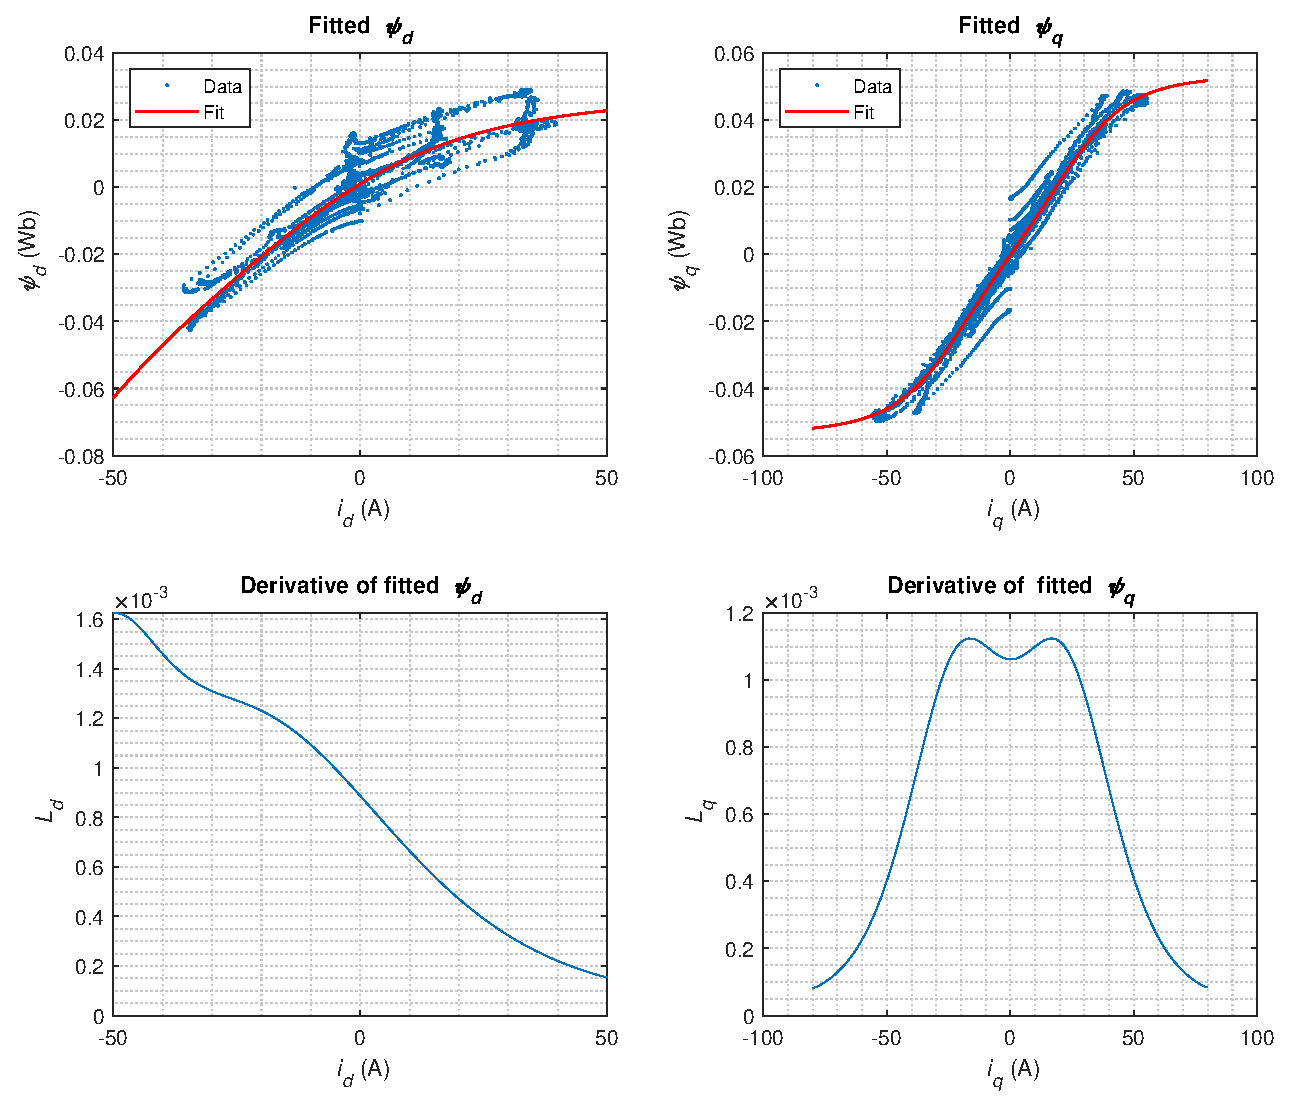
\includegraphics[clip, trim=11.1cm 0cm 0cm 10.1cm,width=0.45\linewidth]{Figures/Ldq.eps}}
	\end{subfigmatrix}
	\caption{Machine Inductance as the current derivative of the flux linkage.}
	\label{fig:inductances}%chktex 24
\end{figure}

\section{Current References}

To simplify the real-time computations, the current references can be calculated offline. A simple approach would be to only consider the quadrature current $i_q$ as the main component of torque, and compute the reference using the torque constant. This approach is simple and fast, but it does not account for the motor's inductance, which can be used to increase efficiency. The maximum torque per ampere strategy actively uses the inductance differences between the direct and quadrature axes to get the maximum torque for a given current, but as the inductances are variable, the optimal current reference is also variable. Although it is possible to use the MPC to optimize the current references, doing it offline not only allows for faster computational times but also results in more precise references. The downside of this approach is that it negates the possibility of acting upon online parameter estimation, however, this drawback can be mitigated by implementing regular calibration procedures.

Using \Cref{eq:motor_with_inductances_no_derivative} and assuming a steady state, a constrained minimization problem can be written to minimize the current modulus with constraints to ensure the reference torque is achieved and to account for back EMF related voltage limitations. This problem is presented in \Cref{eq:mtpa_problem_with_voltage_constraint}.

\begin{equation}
	\begin{aligned}
		\min_{i_d,i_q} \quad & \sqrt{i_q^2 + i_d^2} \\
		\rm{s.t.}  \quad & T_{ref} = p\, i_q((L_d - L_q)i_d + \psi_{PM})\\
		               \quad & {(r i_d -\omega_e \psi_q)}^2 + {(r i_q + \omega_e (\psi_{PM} + i_d L_d))}^2\leq V_{DC}^2            \\
	\end{aligned}
	\label{eq:mtpa_problem_with_voltage_constraint} %chktex 24
\end{equation}

As the solution to this problem is not trivial, the optimization was solved using a numerical approach in \textit{MATLAB}. The resultant current references for the nominal battery voltage are shown in \Cref{fig:mtpa_constrained}.


\begin{figure}[!htb]
    \centering
    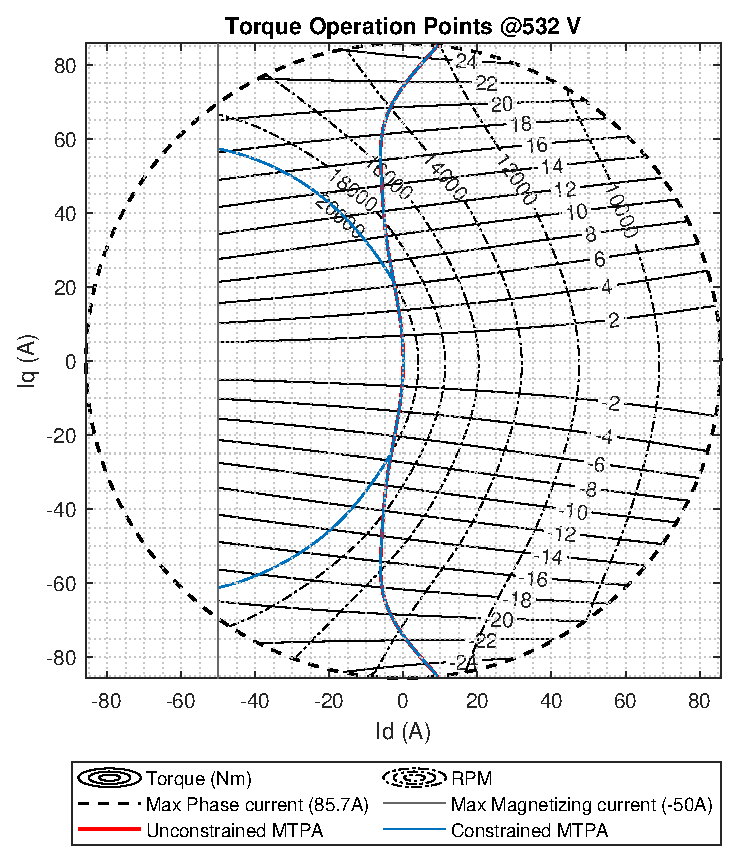
\includegraphics[width=0.8\linewidth]{Figures/Motor_map@532V}
	\caption{Constrained Maximum Torque per Ampere curve at nominal battery voltage. Reference currents are shown for 0, 13000 and 2000 RPMs.}
	\label{fig:mtpa_constrained}%chktex 24
\end{figure}

\section{Proposed Control Strategy}
The proposed control strategy is a Model Predictive Control (MPC) with a horizon of 1 timestep, that uses \Cref{eq:motor_with_inductances_discrete} to evaluate the best possible voltage vector to apply to the motor. One of the advantages of the approximations made in the discretization process is that even though the matrices change in time, for a given moment the system is linear, and as such an inverse dynamic can be derived. So, if in \Cref{eq:motor_backward_euler_matrix} the currents on the next step are replaced by a reference for the current vector, the necessary applied voltage can be calculated:

\begin{equation}
	\begin{aligned}
		\begin{bmatrix}
			u_{d(k+1)} \\
			u_{q(k+1)} \\
		\end{bmatrix}
		=
		\begin{bmatrix}
			\frac{h}{hr+L_{d(i_d(k))}} & 0                          \\
			0                          & \frac{h}{hr+L_{q(i_q(k))}} \\
		\end{bmatrix}^{-1} \\
		\left(
		\begin{bmatrix}
				1                                                    & -h\frac{\omega_{e(k)}L_{q(i_q(k))}}{hr+L_{d(i_d(k))}} \\
				h\frac{\omega_{e(k)}L_{d(i_d(k))}}{hr+L_{q(i_q(k))}} & 1                                                     \\
        \end{bmatrix}
		\begin{bmatrix}
				i_{d_{ref}} \\
				i_{q_{ref}} \\
        \end{bmatrix}
        \right. -\\-
		\begin{bmatrix}
				\frac{L_{d(i_d(k))}}{hr+L_{d(i_d(k))}} & 0                                      \\
				0                                      & \frac{L_{q(i_q(k))}}{hr+L_{q(i_q(k))}} \\
        \end{bmatrix}
		\begin{bmatrix}
				i_{d(k)} \\
				i_{q(k)} \\
        \end{bmatrix}
        -\\- \left.
		\begin{bmatrix}
				0                                                 \\
				-h\frac{\omega_{e(k)}\psi_{PM}}{hr+L_{q(i_q(k))}} \\
			\end{bmatrix}
		\right)
	\end{aligned}
\end{equation}

This approach is commonly used in linear unconstrained MPCs to improve computation times, where a control law is precomputed and stored in memory. But in the presented case there is an important constraint that is not accounted for in the previous equation. When very short time steps are used, and there is a big reference change, the necessary voltage to achieve the target on just one discrete time step can be very high. This would lead to problems, like distortions due to overmodulation or not being able to reach the desired voltages. The solution to this problem is to saturate the voltage vector. Some authors have suggested saturating based on the closest possible vector~\cite{Fernando:fast_predictive:2013}, in this work, the saturation only limits the vector amplitude to match the DC-link voltage, maintaining the desired vector angle as shown in \Cref{eq:Vdq_saturation}.
\begin{subequations}
	\begin{equation}
			\gamma = arctg\left(\frac{u_{d(k+1)}}{u_{q(k+1)}}\right)
	\end{equation}
	\begin{equation}
		u_{sat_{d(k+1)}} = \min\left(u_{d(k+1)}\;,\; V_{dc}\cos(\gamma)\right)
	\end{equation}
	\begin{equation}
		u_{sat_{q(k+1)}} = \min\left(u_{q(k+1)}\;,\; V_{dc}\sin(\gamma)\right)
	\end{equation}
	\label{eq:Vdq_saturation}
\end{subequations}

% \begin{figure}[!htb]
% 	\centering
% 	\includegraphics[width=1\linewidth]{Figures/Explicit_CSMPC.pdf}
% 	\caption[Explicit Continuous Set MPC Diagram.]{Explicit Continuous Set MPC Diagram.}
% 	\label{fig:explicit_csmpc_diagram}%chktex 24
% \end{figure}

This method greatly reduces the time taken to compute the control action, as instead of trying 7 different possible inputs (or more) it just calculates one time the necessary voltage and clamps it to the attainable values. As this control uses a continuous set, those values are then forwarded to an SVM system to modulate the Pulse Width Modulation (PWM) signals.

\section {Horizon Extension}

A previously overlooked problem is the compensation of the computational time, as the acquisition and control calculations cannot be done instantly their delay needs to be compensated. The strategy adopted here is to use the motor model equations \Cref{eq:motor_backward_euler_matrix} coupled with the previously calculated control action to predict the system state in the next time step. Usually, this is done in a fixed timestep manner, where the predictive controllers instead of picking the control action for $k$ in the timestep $k$, pick the control action for $k+1$ in the timestep $k$, as shown in \Cref{eq:horizon_default} where $x$ represent the currents, $u$ is the voltage vector, $A$, $B$, $C$, and $D$ are the matrices and vectors of the model in \Cref{eq:motor_backward_euler_matrix} and are all dependent on the prediction duration $h = \frac{1}{f_{sw}}$.
\begin{equation}
	x_{k+1} = A^{-1} \left (B x_k + C u_k + D\right )
	\label{eq:horizon_default}
\end{equation}
For this equation to work the system timeline needs to be as in \Cref{fig:horizon_default_timeline}, starting with taking the current and voltage measurements, followed by applying the voltage vectors calculated in $k-1$, then extending the horizon by one timestep, and calculating the voltage vector for the next timestep~\cite{Vazquez:MPC_uses:2014}.

\begin{figure*}[!htb]
	\centering
	\includegraphics[width=.8\linewidth]{Figures/Horizon Extension default Timeline.pdf}
	\caption[Horizon extension by one timestep.]{Horizon extension by one timestep.}
	\label{fig:horizon_default_timeline} %chktex 24
\end{figure*}

This can be improved by only extending the horizon by the necessary time to compute the control action, this way the prediction error derived from model mismatch is reduced because the amount of time to predict is smaller. To do that the prediction duration is simply reduced to $h = t_{control}$, while the system timeline is shifted as in \Cref{fig:horizon_extend_timeline}. The combination of explicitly solving the MPC model equation with the hybrid horizon timestep approach, where the horizon extension has a shorter timestep than the controllable horizon is called Real-time Ultra Short Horizon extension MPC (RUSH MPC). It has the benefits of being a continuous set model predictive control, thus reducing the ripple, while being computationally efficient, as it is explicitly calculated, and reducing the prediction error due to model mismatch as it uses the reduced horizon extension technique.

\begin{figure*}[!htb]
	\centering
	\includegraphics[width=.8\linewidth]{Figures/Horizon Extension Timeline.pdf}
	\caption[Horizon Extension by control time.]{Horizon Extension by control time.}
	\label{fig:horizon_extend_timeline} %chktex 24
\end{figure*}

The final control cycle starts with sensor acquisition, followed by horizon extension, and lastly the future control action computation. Note that this delay is not a problem with simulation in \textit{Simulink}, as it can instantly do the calculations, but it is good practice to simulate it with the proper delays to increase the similarity between simulation and experimental results.

\section{Simulation}
\label{section:simulation}%chktex 24

To accelerate the development time, a model was developed in \textit{Simulink}, allowing for faster prototyping and direct comparison of the methods in a controlled environment. An adaptation of the \textit{Simscape Specialized Power Systems} block \textit{Permanent Magnet Synchronous Machine} was made to convert it to a delta-wound machine and to accept variable inductances as in \Cref{eq:motor_backward_euler_matrix}. 
This model was combined with six MOSFET blocks in three legs to simulate the VSI. To supply the MOSFETs, a model of the battery was made, where an ideal voltage source is connected through a series resistor to the DC link, where a capacitor stabilizes the voltage. In \Cref{fig:simulation_model} the resultant system is presented, where $S_1$, $S_2$, $S_3$, $S_4$, $S_5$, $S_6$, are the gate control signals that come from the control strategy.

\begin{figure*}[!htb]
	\centering
	% \fbox{
		\includegraphics[clip, trim=0.3cm 5cm 0.5cm 5cm, width=.8\linewidth]{Figures/motor_and_inverter_simulink1.pdf}
		% }
	\caption[Simulink Models, Motor and Inverter.]{Simulink Models, Motor and Inverter.}
	\label{fig:simulation_model} %chktex 24
\end{figure*}

\subsection{Baseline Step}
With the model implemented on \textit{Simulink}, a baseline was made using the manufacturer control scheme, FOC with the standard $8kHz$ switching frequency, and compared with the proposed methods at $50kHz$. The difference in frequency is to account for the complete system, where the use of wide bandgap semiconductors allowed for a faster switching frequency. The baseline profile is a positive torque step with the machine fixed at the nominal speed of $12kRPM$. The rising time of each method is shown in \Cref{fig:rising_time_4_models}.
\begin{figure*}[!htb]
	\centering
    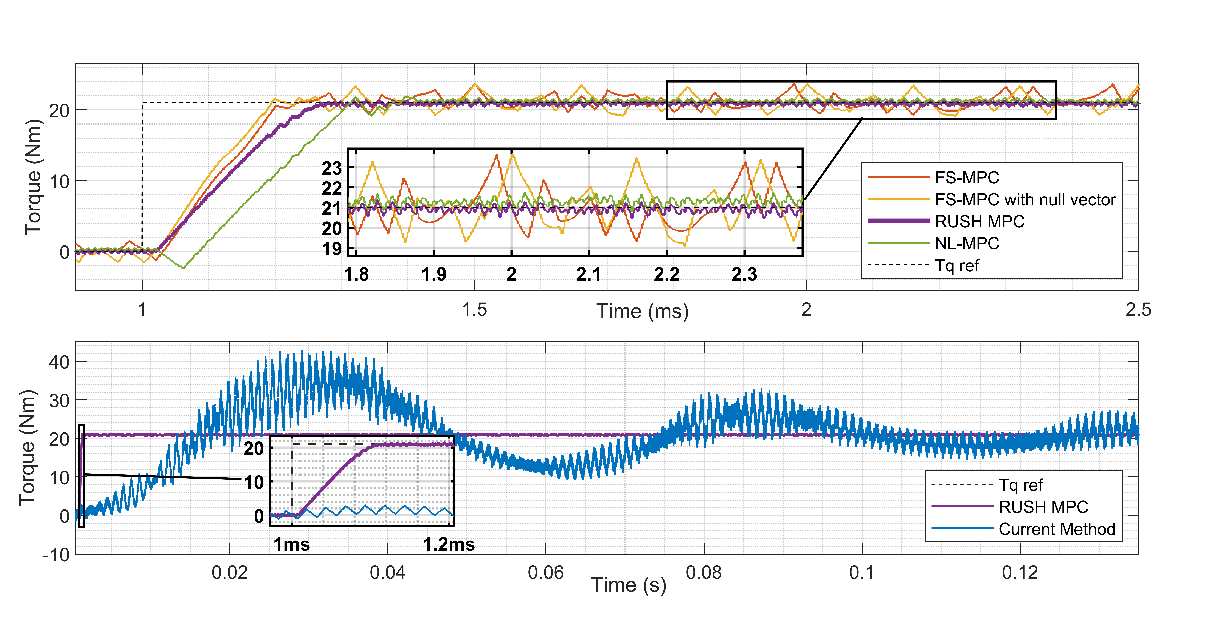
\includegraphics[clip, trim=0cm 0cm 0cm 5.5cm,width=.8\linewidth]{Figures/Step_@12000RPM.eps}
	\caption[Control methods comparison in a torque step.]{Control methods comparison in a torque step. Proposed method (in purple) vs Currently used method (in blue).}
	\label{fig:rising_time_4_models} %chktex 24
\end{figure*}

Note that the predictive controller presents a rising time (0 to 100\%) of $200\mu s$, while the FOC method performed much slower, at approximately $180ms$. While the rising time in the FOC can be improved by better tunning the PID (these results are with the values recommended by the manufacturer), it would result in more pronounced overshoots and settling time, and would not reach the performance of a predictive controller, where the torque rising is only limited by the machine inductances, which shows the great dynamic performance of predictive controllers.

\subsection{Current THD}

The distortion of currents was evaluated by setting the motor at a constant speed, waiting a few periods for it to reach a steady state and then calculating the average THD of all line currents through 5 electrical periods. This was repeated in a grid pattern with some of the results shown in \Cref{table:thd_comparison}.

\begin{table}[h]
	\caption{Control Method Current THD comparison. THD is calculated until the Nyquist frequency, that is $250kHz$ and $40kHz$ for the controllers running at $50kHz$ and $8kHz$ respectively.}
	\label{table:thd_comparison}%chktex 24
	\renewcommand{\arraystretch}{1.2} % more space between rows
		\centering
		\resizebox{1\linewidth}{!}{%
		\begin{tabular}{lrcccc}
			\textbf{} &
			  \multicolumn{1}{l}{\textbf{}} &
			  \textbf{1000 RPM} &
			  \textbf{7333 RPM} &
			  \textbf{13666 RPM} &
			  \textbf{20000 RPM} \\ \toprule
			 &
			  \textbf{1Nm} &
			  57.62\% &
			  43.44\% &
			  207.54\% &
			  29.62\% \\
			 &
			  \textbf{11Nm} &
			  3.22\% &
			  10.62\% &
			  12.14\% &
			  58.53\% \\
			\multirow{-3}{*}{\textbf{\begin{tabular}[c]{@{}l@{}}FOC \\ @8kHz\end{tabular}}} &
			  \textbf{20Nm} &
			  5.15\% &
			  6.50\% &
			  10.18\% &
			  37.08\% \\ \toprule
			 &
			  \textbf{1Nm} &
			  56.95\% &
			  11.08\% &
			  14.12\% &
			  4.71\% \\
			 &
			  \textbf{11Nm} &
			  2.18\% &
			  2.19\% &
			  1.93\% &
			  4.85\% \\
			\multirow{-3}{*}{\textbf{\begin{tabular}[c]{@{}l@{}}FOC \\ @50kHz\end{tabular}}} &
			  \textbf{20Nm} &
			  1.41\% &
			  1.41\% &
			  2.28\% &
			  3.86\% \\ \toprule
			 &
			  \textbf{1Nm} &
			  7.20\% &
			  11.91\% &
			  16.82\% &
			  21.95\% \\
			 &
			  \textbf{11Nm} &
			  0.76\% &
			  1.47\% &
			  1.92\% &
			  2.16\% \\
			\multirow{-3}{*}{\textbf{\begin{tabular}[c]{@{}l@{}}RUSH MPC \\ @50kHz\end{tabular}}} &
			  \textbf{20Nm} &
			  0.81\% &
			  0.98\% &
			  1.19\% &
			  1.12\% \\ \toprule
			 &
			\end{tabular}
		}
\end{table}

Table \ref{table:thd_comparison} exposes the advantage of continuous MPC over the other alternatives, with distortions expressively smaller than the baseline FOC. Another advantage of the proposed method is that it actively uses the direct axis current to generate torque throughout the full operation map of the motor,  not only in field weakening as the method currently implemented on the car. This is a result of the use of Maximum Torque per Apere references which improves efficiency, as it produces a reduction in the current vector modulus necessary to generate the same torque.

\subsection{Robustness}

To test the controller's robustness, a Monte Carlo analysis is proposed. A normal distribution is assigned to the motor parameters with a mean equal to the characterized value, and a standard deviation equal to 5\% of the mean. The step of \Cref{fig:rising_time_4_models} was simulated for 1000 samples with the modified parameters applied to the motor without updating the controller (\Cref{fig:montecarlo}).

% \begin{@twocolumnfalse}
    \begin{figure*}[!htb]
        \centering
        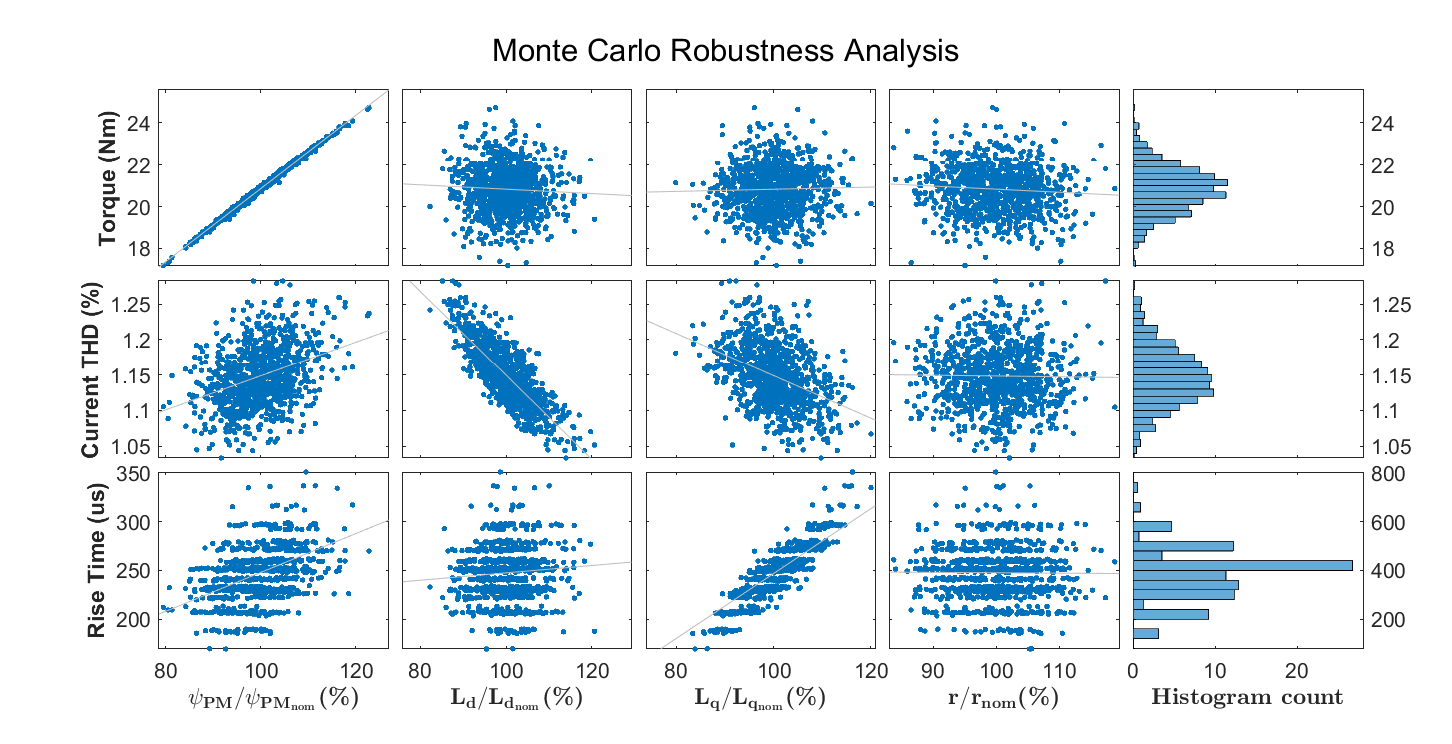
\includegraphics[width=0.8\linewidth]{Figures/MonteCarlo.eps}
        \caption[Monte Carlo Robustness Analysis.]{Monte Carlo Robustness Analysis. The motor parameters are shown in percentual change from the controller's expected value.}
        \label{fig:montecarlo} %chktex 24
    \end{figure*}
% \end{@twocolumnfalse}

To evaluate the performance with degraded parameters three metrics were used, the steady-state mean torque, the steady-state current THD, and the torque rising time. Based on these metrics the most influential parameter is the flux linkage, with a correlation of almost 100\% with the steady-state torque. This is explained by the type of motor used, where the inductances between the direct and quadrature axes are very similar, resulting in most of the torque derived from the permanent magnet's flux linkage. Note that this dependency is also present in the method currently used by the manufacturer, where the quadrature current reference is based on the machine torque constant ($k_t$). 
While relatively easy to characterize, the flux linkage is also the parameter most prone to change with the life of the motors, where the magnets can overheat or be demagnetized by a high direct axis current, thus a good approach is to develop a characterization routine that can be automatically executed whenever the user deems necessary.

The quadrature inductance has a higher correlation with the torque rise time, as expected. Since almost all of the torque is derived from the permanent magnet's flux linkage the torque will rise as fast as the controller manages to create quadrature currents. While this correlation is not definitive proof, it reinforces the statement that the proposed controller dynamic response is limited by the machine inductances. The high flux linkage correlation with the rise time is due to the increase in steady-state torque since with higher flux the steady-state torque is higher and the rise is approximately linear, with an increase in steady-state torque the rise time also increases.

Regarding the current THD, the parameter influences are well balanced, with the direct axis inductance being a little more correlated. When combining this with the small absolute variance of the THD, it is clear that the control strategy is very robust against model mismatches, maintaining a low distortion even with the wrong parameters.

\subsection{Acceleration Event}
\label{section:acceleration}%chktex 24

A load profile that simulates the car environment was used to simulate a typical acceleration event. The torque reference was set to reach $21.3kW$ of delivered power (after inverter and motor efficiency losses), this value was chosen assuming an $80\%$ powertrain efficiency and an approximation of one-third of the car load on the rear motors. As shown in \Cref{fig:acceleration_comparison}, the RUSH MPC improved the time from $3.943s$ to $3.883s$ (\textit{1.6}\%), reaching also a higher top speed than the currently implemented control method and presenting a lower torque ripple.
\patchcmd{\subfigmatrix}{\hfill}{\hspace{0.2cm}}{}{}
\begin{figure*}[!htb]
	\centering
	\begin{subfigmatrix}{2}
		\subfigure[Torque profile in the acceleration event using the currently implemented FOC.]{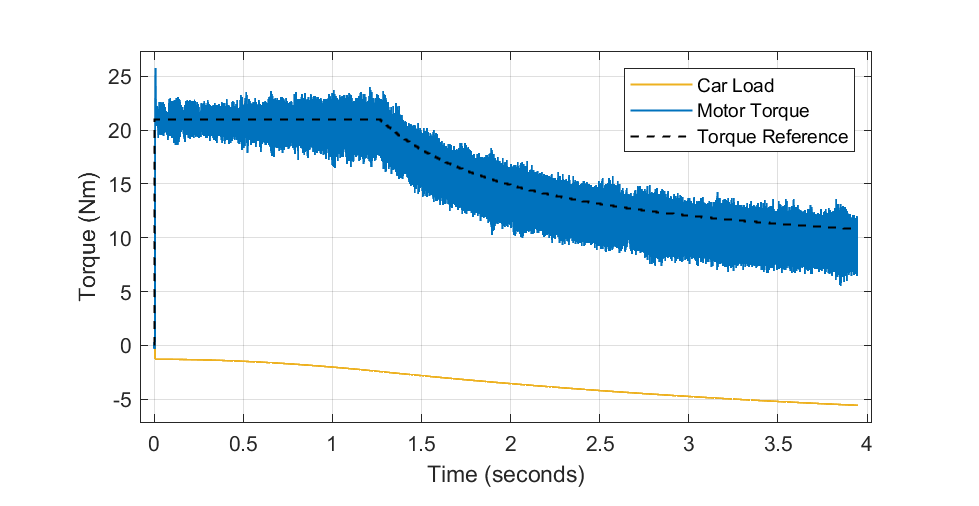
\includegraphics[clip,trim = 1cm 0 1.55cm 0,width=0.4\linewidth]{Figures/acc_empc.eps}\label{fig:acc_foc}}
		\subfigure[Torque profile in the acceleration event using the proposed RUSH MPC]{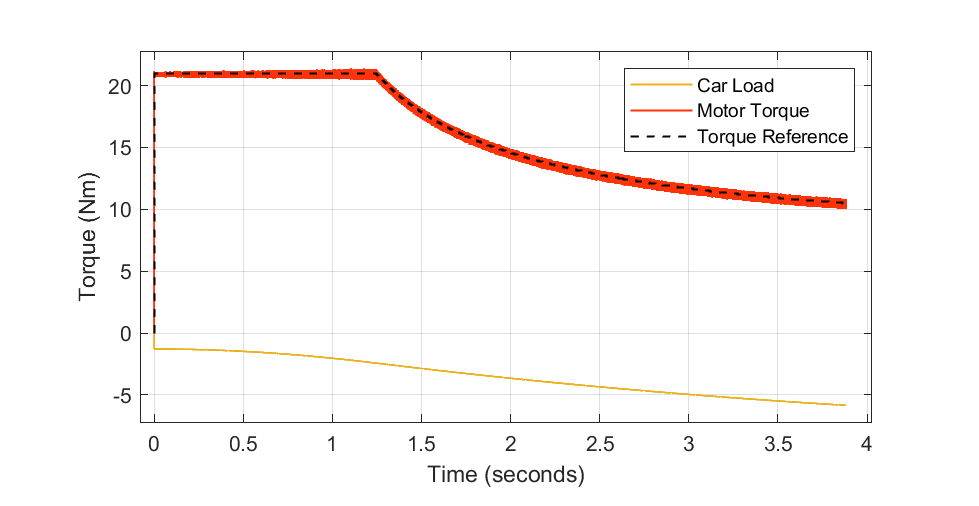
\includegraphics[clip,trim = 1cm 0 1.55cm 0,width=0.4\linewidth]{Figures/acc_foc.eps}\label{fig:acc_empc}}
	\end{subfigmatrix}
	\begin{subfigmatrix}{2}
		\subfigure[Motor speed profile in the acceleration event. The blue line is the currently implemented FOC while the orange line is the proposed RUSH MPC.]{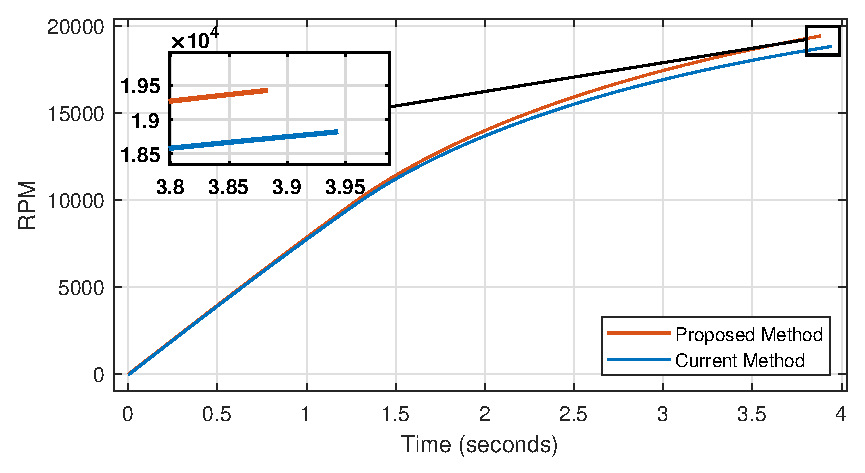
\includegraphics[width=0.4\linewidth]{Figures/acc_rpm.eps}\label{fig:acc_rpm}}
		\subfigure[Distance traveled in the acceleration event. The blue line is the currently implemented FOC while the orange line is the proposed RUSH MPC.]{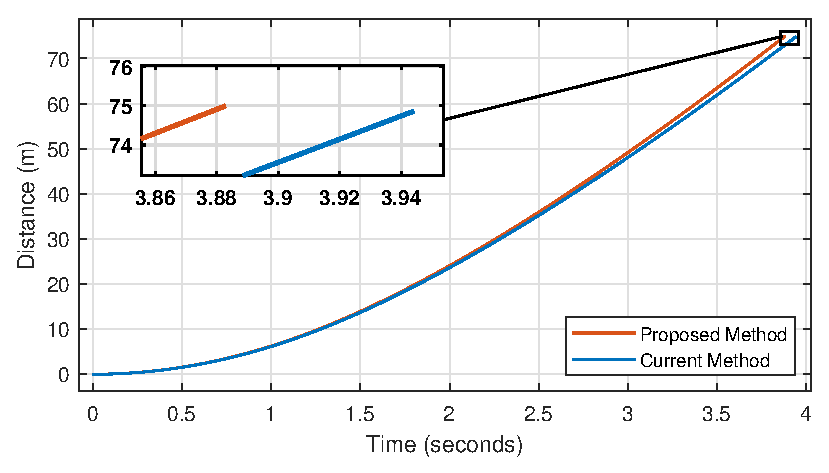
\includegraphics[width=0.385\linewidth]{Figures/acc_dist.eps}\label{fig:acc_dist}}
	\end{subfigmatrix}
	\caption[Control methods comparison on an Acceleration event.]{Control methods comparison on an Acceleration event.}
	\label{fig:acceleration_comparison} %chktex 24
\end{figure*}
\patchcmd{\subfigmatrix}{\hspace{0.2cm}}{\hfill}{}{}

\section{Experimental Results}
\label{section:simulation}%chktex 24

To validate the simulated results, some tests were made on a test bench. The controller was implemented using Xilinx Model Composer inside Simulink, compared with the simulation implementation and then generated for the FPGA present in a Digilent Zybo Z7-20. The hardware used was comprised of the inverter developed on~\cite{Costa:MSc}, coupled with a current measuring board, developed for this thesis to increase noise immunity. The characterized AMK motor was set in a test bench with a Sensor Technology torque transducer (RWT441-EC-PG) and another AMK motor as load.

First, a simple constant torque test was made to evaluate if the model was correctly calculating the generated torque. \Cref{fig:constant_tq} presents the torque estimated based on the motor parameters and the current measurements with the value measured with the ST transducer output. The current measurement had some outliers from Electromagnetic Interference (EMI), so the currents and torque in this section were filtered using a Median Absolute Deviation (MAD) outlier filter.

\begin{figure}[!htb]
	\centering
	\includegraphics[width=1\linewidth]{Figures/constantTq.eps}
	\caption[Torque estimation vs Measured. In the bottom the percentual error between the measured and estimated torques is shown.]{Torque estimation vs Measured. At the bottom, the percentual error between the measured and estimated torques is shown.}
	\label{fig:constant_tq} %chktex 24
\end{figure}

The estimated torque is constantly smaller than the measured torque, with a difference of 0.5Nm. This difference is due to the motor parameters not being perfectly matched with the real motor, and the current measurements not being perfect. The difference between the estimated and measured torque is small enough to consider the model valid for the next tests.

The next step was to verify the current waveform. Ideally, this would be done with nominal torque, but due to a limited maximum inverter current, the motor was commanded to keep a constant torque of $7Nm$. To create a load, the phases of the other motor were short-circuited, creating a load torque that changes with the speed, this resulted in the speed stabilizing at $269RPM$. The current was measured with the developed measuring board and with an oscilloscope probe (ELDITEST CP6550), while the torque was estimated by the control algorithm and compared with the simulation results. The simulation results were obtained by running the same model used for the controller implementation, with the same parameters and inputs. The results are presented in \Cref{fig:tq_step_fig}.
% \begin{figure}[!htb]
% 	\begin{subfigmatrix}{2}
% 		\subfigure[Meausurement Board and Simulation measurements. The plot on top present values from the measurement board, while the bottom plot is from the simulation.]{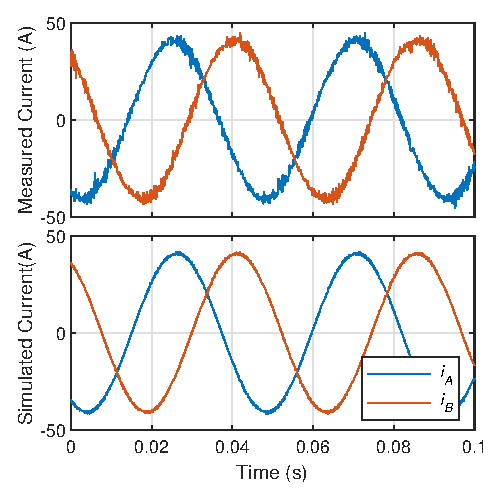
\includegraphics[width=0.47\linewidth]{Figures/const_curr_7NM.eps}\label{fig:steady_state_curr_sim_meas}}
% 		\subfigure[Osicloscope measurements. Channel 1 (in yellow) represents the line A current, while channel 2 (in blue) is the line B current]{\includegraphics[width=0.52\linewidth]{Figures/const_curr_osc_7nm-01.eps}\label{fig:steady_state_curr_osc}}
% 	\end{subfigmatrix}
% 	\caption{Line currents measurements at steady state. Torque reference at $7Nm$ and rotor speed stable at $169RPMs$.}
% 	\label{fig:steady_state_curr} %chktex 24
% \end{figure}

 The oscilloscope measurement was made with a probe that has a sensitivity of $20mV/A$. The results show that the current measured by the developed board is identical to the one from the oscilloscope probe, proving the system's accuracy. When comparing the measured currents with the simulation results, although they have the same form and amplitude, it is clear that the simulated curve is cleaner. This is backed by the THD comparison, where the measured current has a THD of $2.44\%$ and the simulated current has a THD of $0.47\%$, both of them calculated to the 50th harmonic. This difference is due to inaccuracies in the measurements and parametrization. 
 The currents presented in \Cref{fig:tq_step_fig} also show an almost instantaneous dynamic response, transitioning to the specified amplitude without noticeable distortions. The difference between the measured and simulated currents is small enough to consider the model valid.
\begin{figure}[!htb]
	\begin{subfigmatrix}{2}
		\subfigure[Meausurement Board and Simulation measurements. The plot on top presents values from the measurement board, while the bottom plot is from the simulation.]{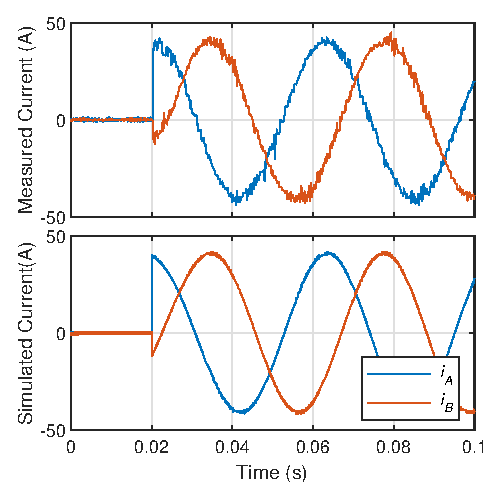
\includegraphics[width=0.465\linewidth]{Figures/tq_step_curr.eps}\label{fig:tq_step_curr}}
		\subfigure[Osicloscope measurements. Channel 1 (in yellow) represents the line A current, while channel 2 (in blue) is the line B current]{\includegraphics[width=0.515\linewidth]{Figures/tq_step_osc-01.eps}\label{fig:tq_step_osc}}
	\end{subfigmatrix}
	\caption{Line Current measurements with a reference torque step from $0$ to $7Nm$ at $0.02s$.}
	\label{fig:tq_step_fig} %chktex 24
\end{figure}



\Cref{fig:tq_step_response_time} shows the torque dynamic response to the step. The reduced sampling time creates significant uncertainty in the measurement, but it is possible to state that the torque rise time is less than 200 microseconds, which is a great improvement when compared with the current control method. The simulation results have a greater sampling rate showing that the rise time is smaller than 100 microseconds. An improved sampling frequency would allow for a better comparison between the simulation and experimental results.

\begin{figure}[!htb]
	\centering
	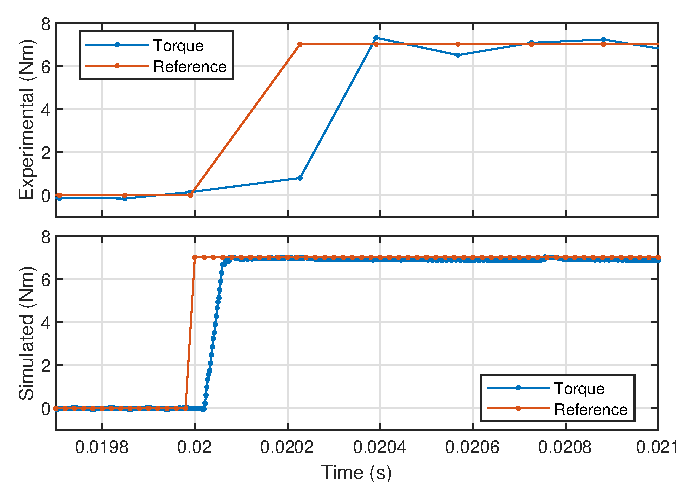
\includegraphics[width=1\linewidth]{Figures/Tq_step.eps}
	\caption[Torque reference follwoing with a step from $0$ to $7Nm$.]{Torque reference follwoing with a step from $0$ to $7Nm$. The upper plot presents the experimental data, while the bottom plot is from the simulation}
	\label{fig:tq_step_response_time} %chktex 24
\end{figure}

To compare the performance of the proposed method, a torque step was also applied to the current solution of the inverter and control strategy. The results presented in \Cref{fig:torque_step_comparison_FOC_MPC} show that as expected, the current solution is much slower than the proposed method, with a rising time of $30ms$ and a delay of $10ms$. 

\begin{figure}[!htb]
	\centering
	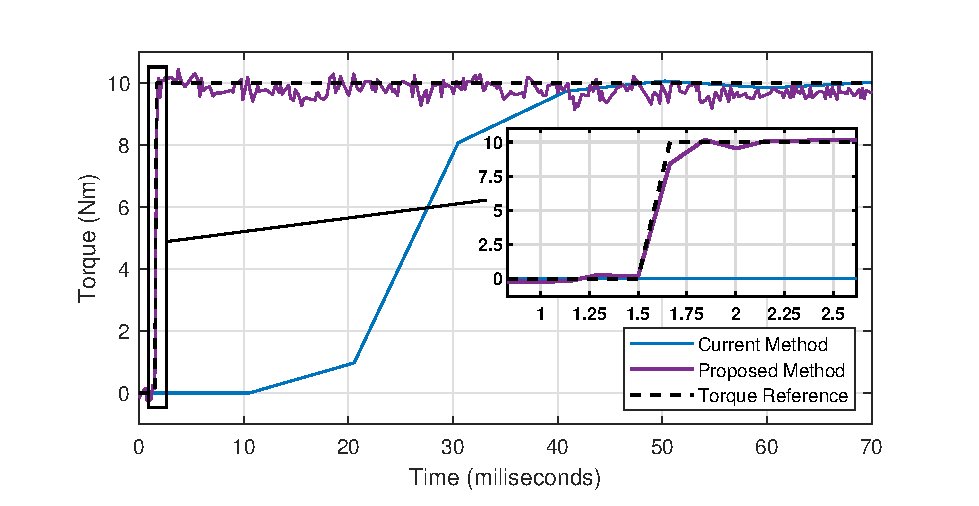
\includegraphics[width=1\linewidth]{Figures/Car_Tq_step.eps}
	\caption{Comparison of torque step response between the proposed method and the currently implemented method.}
	\label{fig:torque_step_comparison_FOC_MPC}%chktex 24
\end{figure}

A torque profile to simulate the driver's input was also tested and is presented in \Cref{fig:pedal_profile}. The controller fails to output the reference torque around $0.1s$ due to the power supply not being able to provide enough current, thus it switched from constant voltage to constant current output, reducing the available voltage to the inverter. Aside from this, the controller was able to follow the torque reference with a small error, averaging $0.04Nm$ and peaking at $1.6Nm$ if the period of the power supply shortage is discarded.
%  A small dependency on the speed can be seen in the torque tracking error, with the error slightly increasing with the rotor velocity. This is seen in the torque ripple increasing, due to the increased back \gls{emf} that requires the controller to increase the modulation index to keep the current amplitude, resulting in saturation

\begin{figure}[!htb]
	\centering
	\subfigure[Line Currents.]{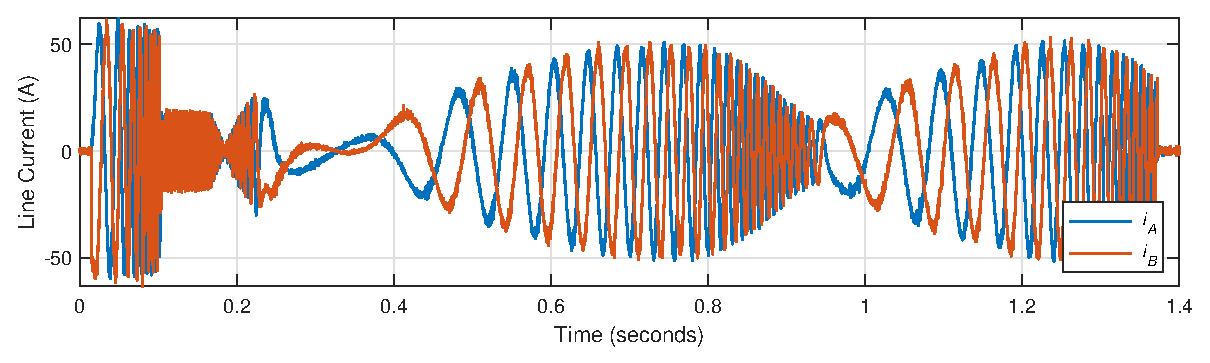
\includegraphics[width=1\linewidth]{Figures/pedal_profile_curr.eps}\label{fig:pedal_profile_curr}}
	\\
	\subfigure[Rotor speed.]{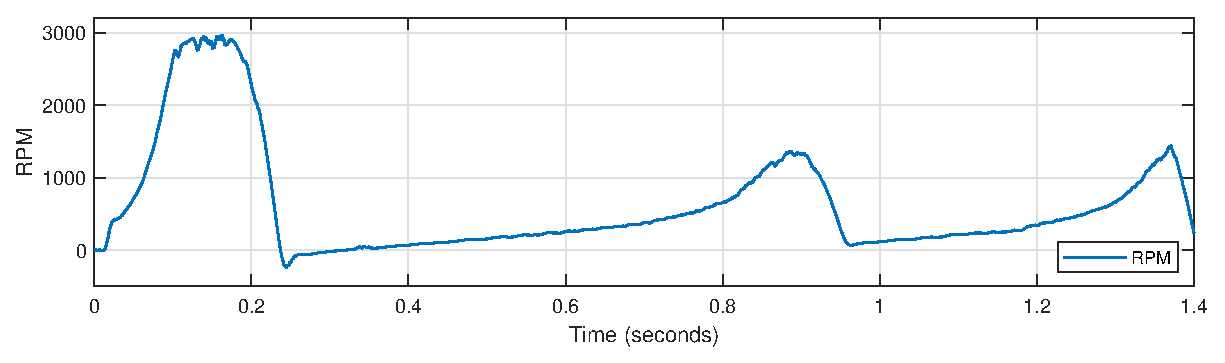
\includegraphics[width=1\linewidth]{Figures/pedal_profile_rpm.eps}\label{fig:pedal_profile_rpm}}
	\\
	\subfigure[Torque reference and measured values. The torque reference is derived from the speed controller but saturated to $\pm 5Nm$.]{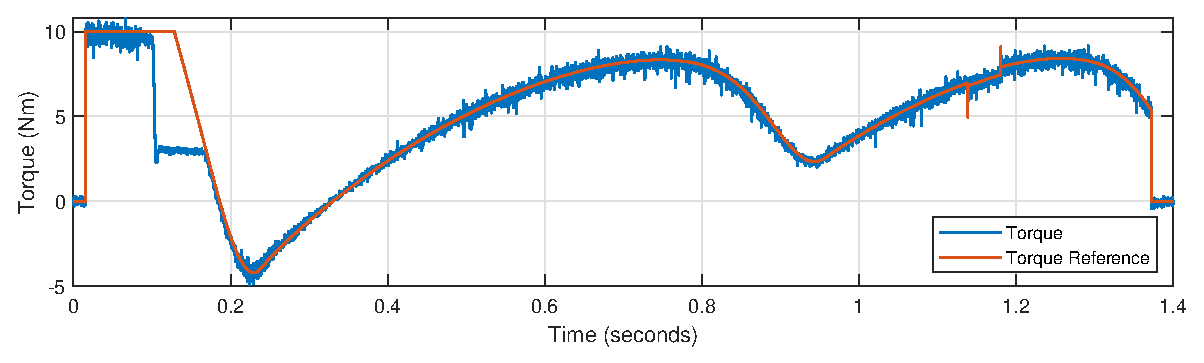
\includegraphics[width=1\linewidth]{Figures/pedal_profile_tq.eps}\label{fig:pedal_profile_tq}}
	\\
	\subfigure[Torque reference tracking error. ]{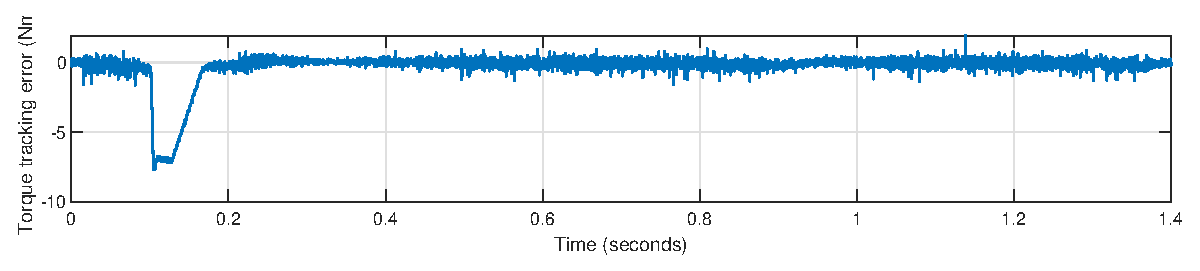
\includegraphics[width=1\linewidth]{Figures/pedal_profile_tq_error.eps}\label{fig:pedal_profile_error}}
	\caption{Pedal torque profile.}
	\label{fig:pedal_profile} %chktex 24
\end{figure}

\section{Conclusions}
\label{chapter:conclusions}
% \minitoc% Creating a minitoc

This work aimed to fill the identified gap in the process of developing a fully in-house powertrain for FST Lisboa which is the control strategy for the motors. This necessity led to a study of control strategies and motor models that was performed with an emphasis on improving the dynamic response of the motor torque and the system efficiency.

To achieve those goals, the motor was characterized by performing several measurements and tests. This not only provided a plant model to simulate the control algorithms but also provided the Formula Student team of Instituto Superior Técnico with valuable information about their motor characteristics and performance.

 With the motor parametrized, it was possible to set up a simulation environment and some control strategies were implemented in it. This allowed a comparison between the different strategies and the selection of the most suitable for the application. The selected strategy was the RUSH MPC due to its fast response, low current ripple, and computational efficiency. 

The proposed control was then implemented in an FPGA and the hardware necessary to test the control in a test bench was developed. The motors and inverter were then assembled on a test bench to perform experimental tests. Although the testbench hardware was later verified to be a limiting factor, the experimental results were very promising.

The simulation and experimental results were compared and analyzed showing a close match between them. The torque estimation was also validated and the control strategy was able to control the motor torque with a dynamic response orders of magnitude smaller than the current solution and with a very low torque ripple. The system efficiency was also improved due to the reduction in current THD.

While not exhaustive the developed system continued to build on the great work of the previous thesis and the team's work, creating a solid platform from which the team can continue the work and implement it on the next prototypes. The work done in this thesis was a major step towards the team's goal of developing a fully in-house powertrain.


\bibliographystyle{./Packages/abbrvunsrtnat_first_name} % <<<<< SELECT IF USING REFERENCES BY NUMBER (CITATION ORDER)
% \bibliographystyle{unsrtnat}
% External bibliography database file in the BibTeX format
\bibliography{Thesis_bib_DB} % file "Thesis_bib_DB.bib"
\def\BibTeX{{\rm B\kern-.05em{\sc i\kern-.025em b}\kern-.08em
    T\kern-.1667em\lower.7ex\hbox{E}\kern-.125emX}}

\end{document}
